\documentclass[final]{beamer}
\usepackage{ragged2e}
\usepackage{wrapfig}

\setbeamertemplate{headline}{
  \leavevmode
  \begin{beamercolorbox}[wd=\paperwidth]{headline}
    \begin{columns}[T]
      \begin{column}{.1\paperwidth}
        %% \vspace{1cm}
        %% 
\includegraphics[width=1\linewidth, keepaspectratio]{./figs/UCLouvain_Logo_Pos_CMJN_prof-eps-converted-to.pdf}\\
        %% \vspace{1cm}
        %% \hspace{1.5cm}
        %% 
\includegraphics[width=.8\linewidth, keepaspectratio]{./figs/LOGO-InstitutDeDuve-Horizontal-CMYK.jpg}
      \end{column}
      \begin{column}{.8\paperwidth}
        \vspace{1cm}
        \usebeamercolor{title in headline}{\color{fg}\textbf{\Huge{\inserttitle}}\\[1.5ex]}
        \usebeamercolor{author in headline}{\color{fg}\huge{\insertauthor}\\[1ex]}
        \usebeamercolor{institute in headline}{\color{fg}\LARGE{\insertinstitute}\\[1ex]}
      \end{column}
      \begin{column}{.1\paperwidth}
        \vskip4ex
      \end{column}
    \end{columns}
  \end{beamercolorbox}

}

\mode<presentation> {  %% check http://www-i6.informatik.rwth-aachen.de/~dreuw/latexbeamerposter.php for examples
}


%% \setbeamertemplate{bibliography item}[text]

\boldmath
\usepackage[orientation=portrait,size=a0,scale=1.85,debug]{beamerposter}                        % e.g. for DIN-A0 poster
%\usepackage[orientation=portrait,size=a1,scale=1.4,grid,debug]{beamerposter}                  % e.g. for DIN-A1 poster, with optional grid and debug output
%\usepackage[size=custom,width=200,height=120,scale=2,debug]{beamerposter}                     % e.g. for custom size poster
%\usepackage[orientation=portrait,size=a0,scale=1.0,printer=rwth-glossy-uv.df]{beamerposter}   % e.g. for DIN-A0 poster with rwth-glossy-uv printer check
% ...
%

%% hide navigation symbols (bottom right)
\setbeamertemplate{navigation symbols}{}

\usepackage{lipsum}
\usepackage{ragged2e}
\usepackage[english]{babel}
\usepackage[latin1]{inputenc}
\usepackage{amsmath,amsthm, amssymb, latexsym}
\usefonttheme[onlymath]{serif}

\usepackage{graphicx}
\usepackage{caption}
\usepackage{subcaption}

\usepackage{listings,lstautogobble}
\lstset{
  language=R,
  basicstyle=\small\ttfamily\color{vdgray}, % the size of the fonts that are used for the code
  % sensitive=false,
  backgroundcolor=\color{lgray},  % choose the background color. You must add \usepackage{color}
  keywordstyle=\color{blue},      % keyword style
  stringstyle=\color{green},      % string literal style
  autogobble=true
}


\usepackage{tcolorbox}
\usepackage{changepage} %% provided adjustwidth
\usepackage{framed}

\newenvironment{Leftbar}{%
  \def\FrameCommand{\vrule width 3pt \hspace{20pt}}%
  \MakeFramed {\advance\hsize-\width \FrameRestore}}%
 {\endMakeFramed}

\newcommand{\R}{\texttt{R} }
\newcommand{\code}[1]{{\texttt{#1}}}
\newcommand{\Rfunction}[1]{{\texttt{#1}}}
\newcommand{\Robject}[1]{{\texttt{#1}}}
\newcommand{\Rpackage}[1]{{\mbox{\texttt{#1}}}}
\newcommand{\email}[1]{\href{mailto:#1}{\normalfont\texttt{#1}}}
\newcommand{\bpkg}[1]{{\textbf{#1}}}

\newcommand{\challenge}[1]{
       \begin{tcolorbox}[notitle,boxrule=1pt,colback=blue!10,colframe=blue!25]
         {#1}
       \end{tcolorbox}
}

\newcommand{\secintro}[1]{
  \bigskip
  \begin{tcolorbox}[notitle,boxrule=10pt,colback=blue!10,colframe=blue!10]{#1}\end{tcolorbox}}

%% colors
\definecolor{Red}{rgb}{0.7,0,0}
\definecolor{Blue}{rgb}{0,0,0.8}
\definecolor{lgray}{rgb}{0.9179688,0.9179688,0.9179688} % #ebebeb
\definecolor{dgray}{rgb}{0.796875,0.796875,0.796875} % #cccccc
\definecolor{vdgray}{rgb}{0.3984375,0.3984375,0.3984375} % #666666
\definecolor{coral}{rgb}{0.9960938,0.4960938,0.3125000} % #ff7f50
\definecolor{blue}{rgb}{0.4218750,0.6484375,0.8007812} % #6ca6cd
\definecolor{green}{rgb}{0.6992188,0.7265625,0.5078125} % #b3ba82
\definecolor{yellow}{rgb}{0.9570312,0.8671875,0.6992188} % #f5deb3

\usepackage{hyperref}
\usepackage{breakurl}
\hypersetup{%
  pdfauthor={Laurent Gatto},%
  pdfusetitle,
  bookmarks = {true},
  bookmarksnumbered = {true},
  bookmarksopen = {true},
  bookmarksopenlevel = 2,
  unicode = {true},
  breaklinks = {false},
  hyperindex = {true},
  colorlinks = {true},
  linktocpage = {true},
  plainpages = {false},
  linkcolor = {Blue},
  citecolor = {Blue},
  urlcolor = {Red},
  pdfstartview = {Fit},
  pdfpagemode = {UseOutlines},
  pdfview = {XYZ null null null}
}


\setbeamertemplate{caption}[numbered]

%% %% figure numering
%% \usecaptiontemplate{
%%   \small
%%   \structure{\insertcaptionname~\insertcaptionnumber:}
%%   \insertcaption
%% }


\title[R for Mass Spectrometry]{\huge The R for Mass Spectrometry Initiative}

\author[Gatto et al.]{
  \large Laurent Gatto$^{1}$, Sebastian Gibb$^{2}$ and Johannes Rainer$^{3}$
}

\institute[]{
  \begin{small}
    $^{1}$ de Duve Institute, UCLouvain, Brussels, Belgium \\
    $^{2}$ Department of Anaesthesiology and Intensive Care, University Medicine Greifswald, Germany \\
    $^{3}$ Institute for Biomedicine, Eurac Research, Italy \\
    ~
  \end{small}
}


\date[]{~}
%% \date{}

\begin{document}

\begin{frame}[fragile]

  \begin{columns}[T]

    \begin{column}{.3\textwidth}

      \begin{block}{}
        \secintro{ \justifying The aim of the \textbf{R for Mass
            Spectrometry} initiative is to provide efficient,
          thoroughly documented, tested and flexible R software for
          the analysis and interpretation of high throughput mass
          spectrometry assays, including proteomics and metabolomics
          experiments.}
      \end{block}

      \begin{block}{}
        \begin{center}
          {\large For more details, visit \\
            \url{RforMassSpectrometry.org}}
        \end{center}

      \end{block}

      \begin{block}{}
        \justifying The project formalises the longtime collaborative
        development efforts of its core members (notably the
        \Rpackage{mzR}, \Rpackage{MSnbase} and \Rpackage{xcms}
        packages) under the \textit{RforMassSpectrometry} organisation
        to facilitate dissemination and accessibility of their work.
      \end{block}


      \begin{block}{}
        \justifying \textit{RforMassSpectrometry} currently contains a
        set of core packages (described on the right), that lay out
        the infrastructure for the \textbf{analysis and interpretation
          of high throughput mass spectrometry assays}.

      \end{block}

      \vspace{2cm}

      \secintro{

        The project is still at an early stage. \textbf{Contributions}
        to the initiative are more than welcome, whether under the
        form of ideas, documentation, code, packages, \ldots \\

        Find details about contribution guidelines and \textbf{code of
          conduct} on our web page.

      }

    \end{column}

    \begin{column}{.2\textwidth}
          \begin{figure}
            \centering
            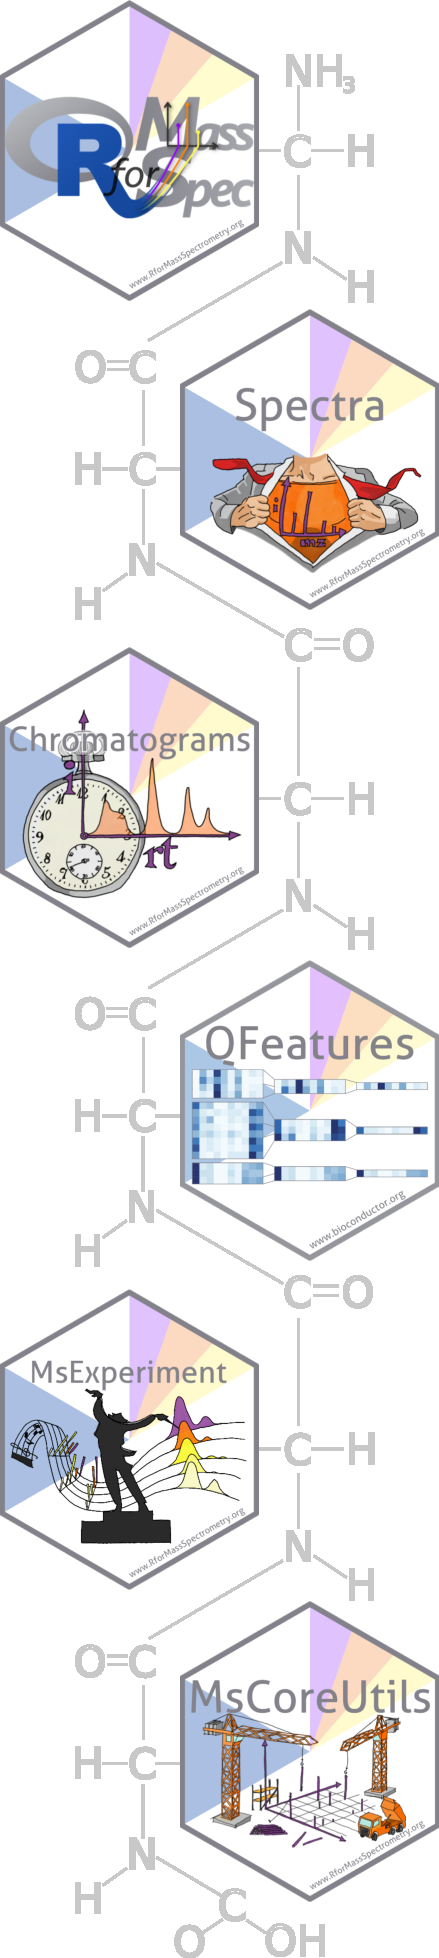
\includegraphics[width=1\linewidth]{./figs/pkgs.pdf}
          \end{figure}

    \end{column}

    \begin{column}{.4\textwidth}

      \begin{block}{}
        \justifying \bpkg{RforMassSpectrometry} is a meta-package that
        is used to manage the R for Mass Spectrometry suite of package
        versions in a coherent way. Users will rely on this package to
        install and manage the other software.
      \end{block}

      \vspace{1cm}

      \begin{block}{}
        \justifying The \bpkg{Spectra} package provides base classes
        and processing methods for raw mass spectrometry data. It is
        designed with efficiency, both in terms of memory footprint
        and processing time in mind, and can manage data in different
        types of formats.
      \end{block}

      \vspace{1cm}

      \begin{block}{}
        \justifying The \bpkg{Chromatograms} package provides base
        classes and processing methods for chromatographic data. It
        is designed with efficiency, both in terms of memory footprint
        and processing time in mind, and can manage data in different
        types of formats.
      \end{block}

      \vspace{1cm}

      \begin{block}{}
        \justifying The \bpkg{QFeatures} package offers the
        infrastructure to manage and process quantitative features for
        high-throughput mass spectrometry assays, including proteomics
        and metabolomics experiments.
      \end{block}

      \vspace{1cm}

      \begin{block}{}
        \justifying The \bpkg{MsExperiment} package provides the
        infrastructure to store and manage all aspects related to a
        complete proteomics or metabolomics mass spectrometry
        experiment. It relies on the other RforMassSpectrometry core
        packages for the data crunching.
      \end{block}

      \vspace{1cm}

      \begin{block}{}
        \justifying The \bpkg{MsCoreUtils} package defines low-level
        functions for mass spectrometry data processing and is
        independent of any high-level data structures.
      \end{block}


    \end{column}

  \end{columns}

  \begin{columns}

    \begin{column}{.7\textwidth}

      \vspace{2cm}

      \begin{block}{}
        To install all the \textbf{R for Mass Spectrometry} packages
        and load the core packages:

        \vspace{5mm}

        \begin{lstlisting}
          BiocManager::install("RforMassSpectrometry/RforMassSpectrometry")
          library("RforMassSpectrometry")
        \end{lstlisting}

      \end{block}
    \end{column}
    \begin{column}{.2\textwidth}
    \end{column}
  \end{columns}

  \vfill


\end{frame}

\end{document}
